\chapter{本提案手法の設計}
\label{proposal}
第\ref{consideration}章では,DynamicEAMTを設計する上で考えられる二種類のアプローチについて,求められる要件に照らし合わせて評価・検討を行った.
本章では検討結果の得られた内容を基に,本研究において提案するDynamicEAMTの実現手法の設計に関して論じる.

\section{概要}
本提案手法では動的経路制御プロトコルであるBGPを利用したサーバー・BR間のメッセージングにより,SIIT-DCネットワークにおけるDynamicEAMTを実現する.
加えて\ref{consideration:approach}で論じた中央管理型・分散管理型の両アプローチの利点を活用可能な,iBGP\footnote{Internal BGP}・RR\footnote{Route Reflector}構成を採用することにより,デプロイメントが容易且つスケーラビリティに優れたメッセージングが可能になる.

\section{BGP}
\subsection{概要}
BGPとはインターネットにおいて自律システム\footnote{Autonomous System. インターネットを構成するネットワークをそれぞれ独立的に運用する組織群を指す.}間の経路情報交換に用いられるパスベクタ型の動的経路制御プロトコルである.現在有効なバージョンはBGP4であり,RFC4271で定義されている\cite{RFC4271}.


\subsection{用語}
BGPにおいて利用される用語のうち,本提案手法において重要なものを以下に列記する.

\subsubsection{BGPスピーカー}
BGPを実装された機器をBGPスピーカーと呼ぶ.

\subsubsection{BGPピア}
BGPで経路交換を行う関係にある機器をぞれぞれBGPピアと呼称する.

そのうち,自律システム間での接続関係にあるBGPピアをEBGP\footnote{External BGP}ピア,同一自律システム内のBGPスピーカー同士の経路交換に用いられるピアをIBGPピアと呼ぶ.

\subsubsection{BGPコネクション}
BGPコネクションとはBGPで経路交換に用いられる接続関係を指す.各機器は1対1の関係でBGPコネクションを確立する.
BGPコネクションにはトランスポート層のプロトコルとしてTCP/179\footnote{TCP\cite{RFC793}のポート番号179}が利用され,フラグメンテーションや再送制御,応答確認,誤り制御等,TCPによる高信頼なメッセージングが可能である.

また,BGPコネクションを維持・管理するために,BGPでは以下のような4つのメッセージが定義されている.

BGPコネクションはBGPピア間でTCPコネクションを確立したのちにOPENメッセージにより各機能の対応関係を確認することにより確立され,KEEPALIVEメッセージによりセッションが維持される.UPDATEメッセージにより,BGPピアへ広告する経路\footnote{Adj-RIB-Out.}に変更が生じたことを通知する.何らかの理由によりBGPコネクションが確立出来なくった場合,NOTIFICATIONメッセージを利用して切断を通知する.

\subsubsection{Adj-RIB-In/Adj-RIB-Out/Loc-RIB}
\begin{figure}[h]
    \begin{center}
    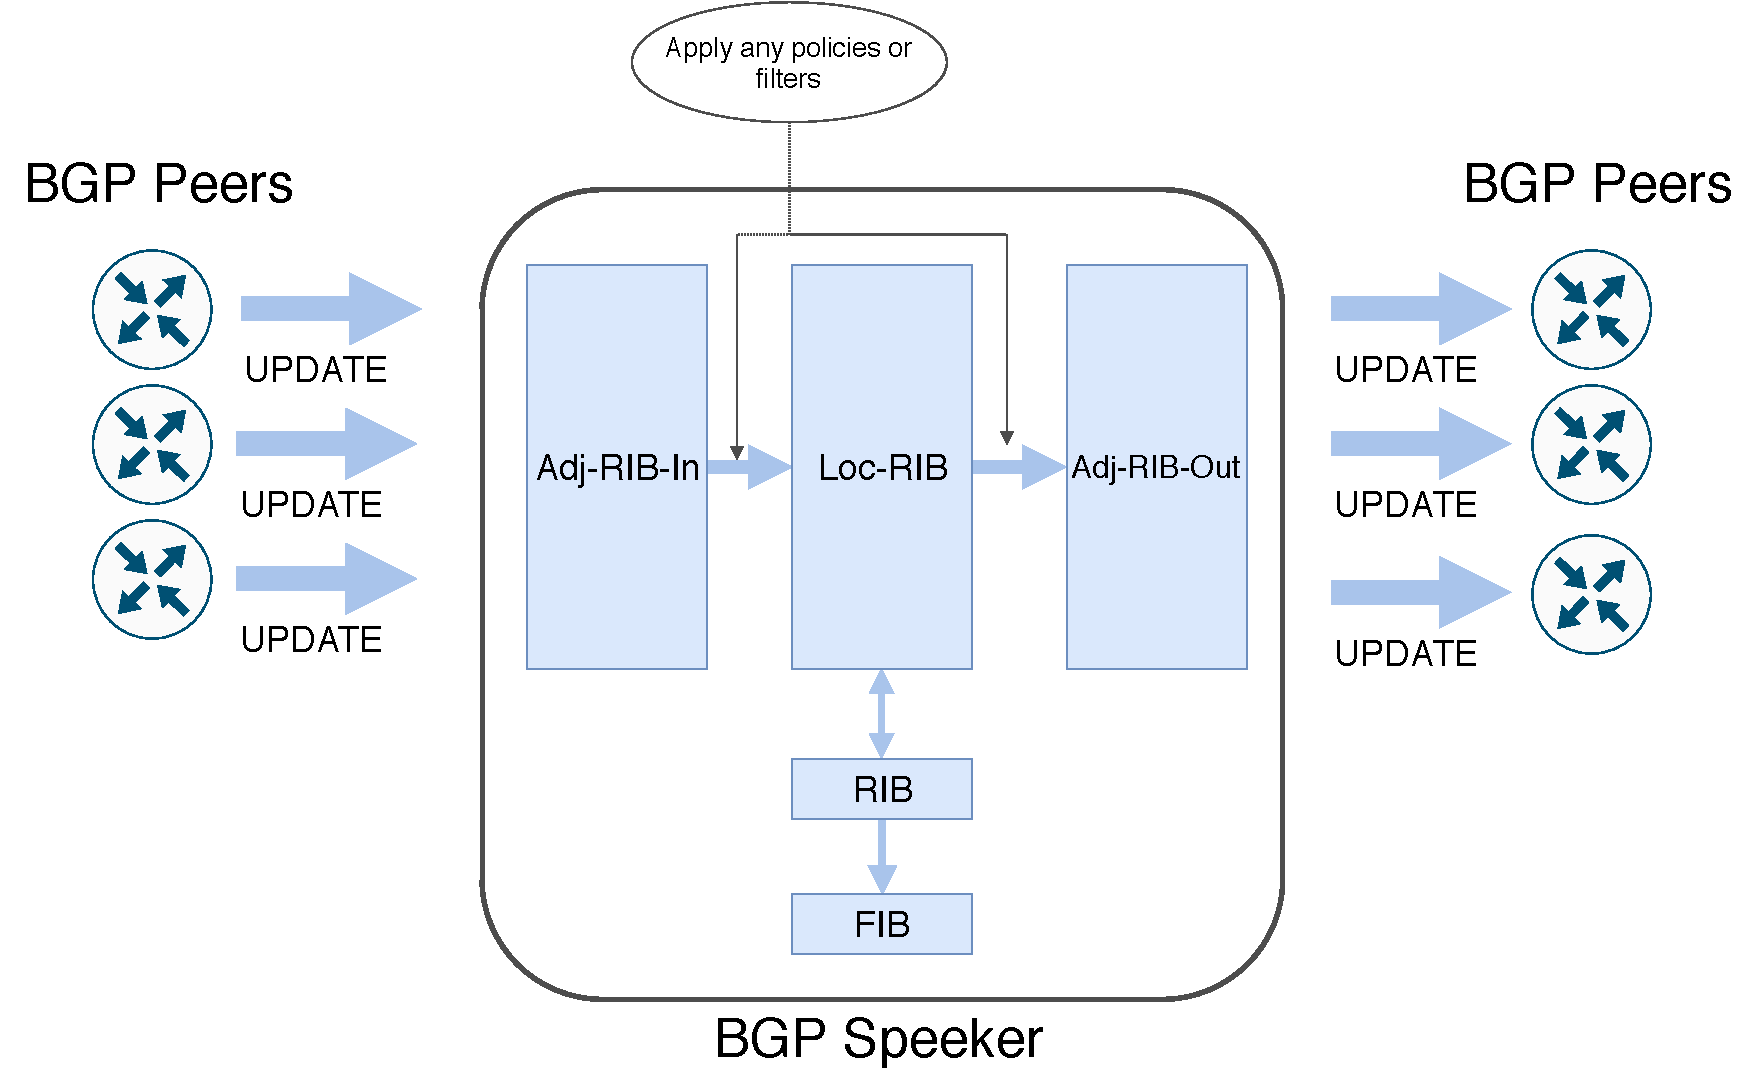
\includegraphics[width=10cm,pagebox=cropbox,clip]{img/bgp-rib-model.pdf}
    \end{center}
    \caption{BGPスピーカーの経路の扱い}
    \label{fig:bgp-rib-model}
\end{figure}
図\ref{fig:bgp-rib-model}にBGPにおける経路受信・保持・送信の流れを示す.
BGPピアから受信した経路はAdj-RIB-Inと呼ばれ,BGPスピーカーの任意のフィルターやポリシーを適用した上でLoc-RIBと呼ばれるテーブルに保存される.
BGPスピーカーはLoc-RIBから任意のフィルターを適用した経路をBGPピアに広告する.この広告する経路をAdj-RIB-Outと呼ぶ.




\subsection{特徴}
本提案手法においてDynamicEAMTを実現するためのメッセージングプロトコルとしてBGPを選択するに至った要素について記述する.

\subsubsection{マルチプロトコル}
現行版であるBGP4では,OPENメッセージにオプション値\footnote{Capabilities Optional Parameter.}を挿入することで,IANAによって定められた任意のネットワークプロトコル\cite{IANA_AFI,IANA_SAFI}の経路を交換することが想定されている\cite{RFC4760}.本提案手法で利用しているIPv6ユニキャスト経路もこの機構により実装されている.


\subsubsection{実装が一般的}
BGPは自律システム間の経路交換プロトコルとしてインターネットで利用されている実質的に唯一のプロトコルであり,OSS\footnote{Open Source Software}にも多くの実装が存在する.
広く普及したプロトコルを利用することにより,特別な実装を最小限にして本提案手法を実現することが出来る.

\subsubsection{中継ネットワークに非依存}
本提案手法で採用しているIBGPでは,TTL\footnote{Time to Live. そのパケットが宛先ホストに到達するまでに許容される中継ルーター数.IPv6プロトコルではHop Limitとして同一の機能が実装されている\cite{RFC8200}.}が255に設定されており,BGPピア間でIPv4/IPv6による到達性があればメッセージングを行うことが可能である.すなわち本提案手法は既存のSIIT-DCネットワークに非依存であり,これは第\ref{consideration:points}項で述べた要件の一つである,デプロイメントの容易さを充足する.


\section{基本的なネットワーク設計}
\label{proposal:network}
\begin{figure}[h]
    \begin{center}
    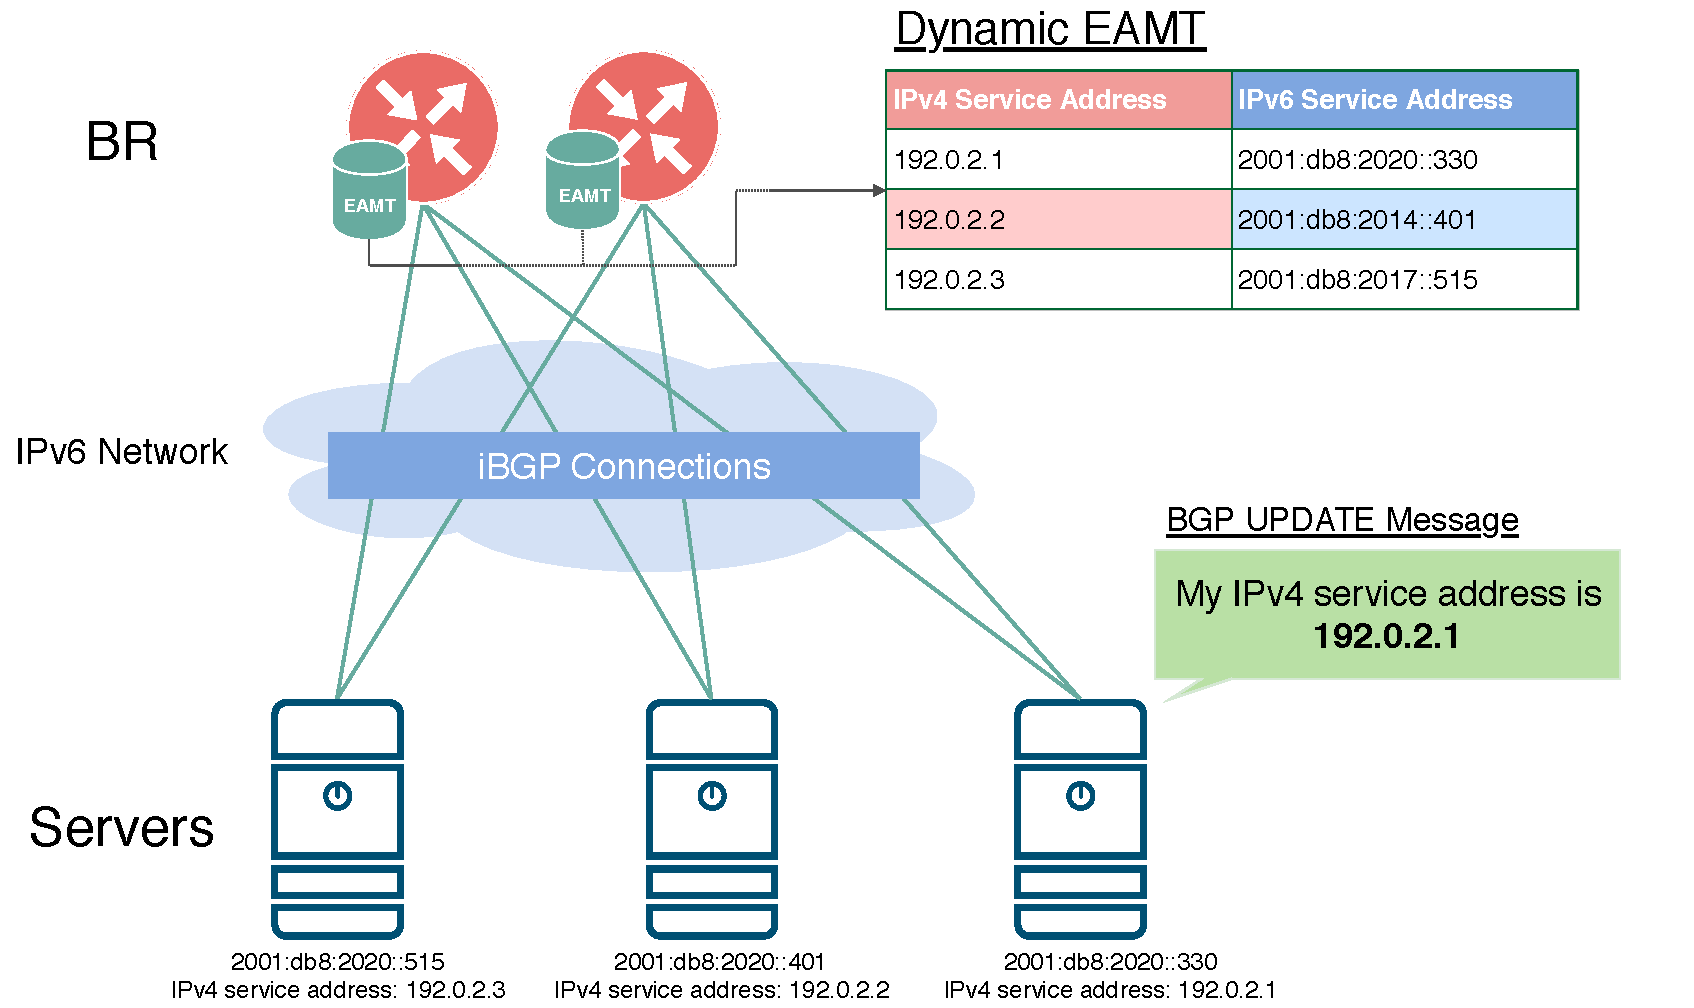
\includegraphics[width=15cm,pagebox=cropbox,clip]{img/proposal_method_network.pdf}
    \end{center}
    \caption{本提案手法の基本機能を実装したSIIT-DCネットワークの例}
    \label{fig:proposal_method_network}
\end{figure}


図\ref{fig:proposal_method_network}本提案手法の各要素の関係を示す.

BR数を$N$,サーバー数を$M$とした,ルートリフレクターを利用した本提案手法での必要なBGPコネクション数$C_a$は以下の様に表現できる.

\begin{equation}
    C_a = M \cdot N
\end{equation}


\subsection{各ノードの役割と機能要件}
\subsubsection{BR}
BRでは下記のような3つの機能が必要となる.
\begin{itemize}
    \item BGPデーモン\\
    各サーバーとiBGPコネクションを確立し,Loc-RIBを生成する.
    \item SIIT機構\\
    EAMTを保持し,それを参照してIPv4/IPv6プロトコル変換を行う.
    \item EAMT制御機構\\
    BGPデーモンが有するのLoc-RIBを参照し,EAMTを更新する.
\end{itemize}

\subsubsection{IPv4サービス提供サーバー}
IPv4サービス提供サーバーでは以下の2つの機構が求められる.
\begin{itemize}
    \item IPv4サービス\\
    IPv4によりインターネットに提供したいサービスを稼働させる.
    \item BGPデーモン\\
    自身が提供するIPv4サービスアドレスを含んだ情報を広告する.
\end{itemize}


\section{ルートリフレクターを活用したネットワーク設計}

\begin{figure}[h]
    \begin{center}
    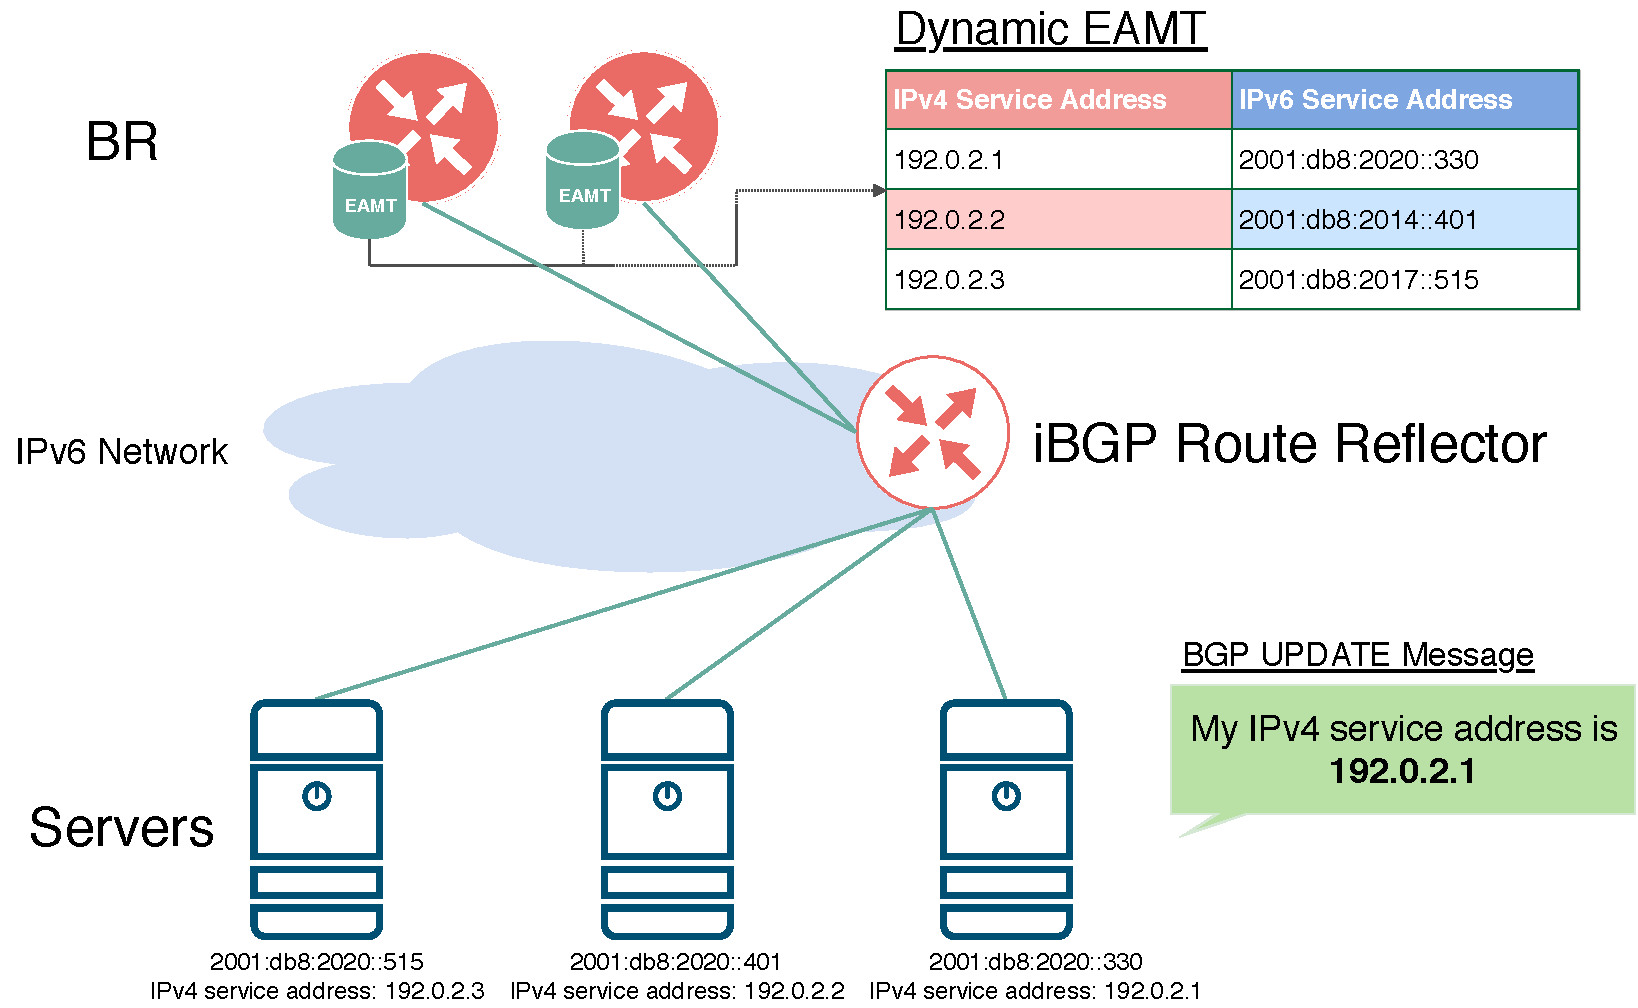
\includegraphics[width=15cm,pagebox=cropbox,clip]{img/proposal_method_network_rr.pdf}
    \end{center}
    \caption{ルートリフレクターを採用したSIIT-DCネットワークの例}
    \label{fig:proposal_method_network_rr}
\end{figure}

通常,iBGPではルートループを防ぐために異なるBGPピアから受信した経路は他のBGPピアに広告されない.そのため一つのiBGPスピーカーが広告する経路を他のiBGPスピーカーが受信するためには,BGPコネクションをフルメッシュで確立する必要がある\cite{vutukuru2005construct}.

ルートリフレクターとは,Originator-IDと呼ばれる特殊な属性をAdj-RIB-Outに付与することでルートループを防ぎながら,iBGPピアから受信した経路を他のiBGPに対して広告する特殊なBGPスピーカーである\cite{RFC4456}.ルートリフレクターはiBGPのコネクション数を削減するために広く利用されている.

ルートリフレクターを複数設置することで,負荷分散・冗長化構成を容易に実現することが出来る.なお,その際ルートリフレクター間はフルメッシュにてBGPコネクションを確立する必要がある.


BR数を$N$,サーバー数を$M$,ルートリフレクターの数を$L$とした,ルートリフレクターを利用した本提案手法での必要なBGPコネクション数$C_b$は以下の様に表現できる.
これはSIIT-DCネットワークが大きくなった場合に,フルメッシュ構成での\ref{fig:proposal_method_network_rr}と比較して,ネットワークへの負荷軽減に大きく繋がる.

\begin{equation}
    C_b = \frac{L(2M + 2N + L - 1)}{2} 
\end{equation}


\subsection{各ノードの役割と機能要件}
\subsubsection{BR及びIPv4提供サーバー}
BR及びIPv4サービス提供サーバーは,ルートリフレクターとのみBGPコネクションを確立する.複数ルートリフレクターを配備する場合,それぞれとコネクションを確立することで冗長性を高めることが出来る.
その他の機能は第\ref{proposal:network}で述べたものと同様に配備する.

\subsubsection{ルートリフレクター}
ルートリフレクターでは,ルートリフレクター機能が有効となったBGPデーモンを配備する必要がある.各サーバー・BRとBGPコネクションを確立する.


\section{各アプローチとの比較}
第\ref{consideration:approach}節で検討した各アプローチと本提案手法を,第\label{consideration:points}節で挙げた各性能要件に関して比較する.

表\ref{table:compare_approach}にそれぞれの項目における比較結果を表す.なお,コントローラーもしくはルートリフレクターの導入数を$L$,サーバー数を$M$,BRの数を$N$としている.



\begin{table}[h]
    \resizebox{\textwidth}{!}{%
    \begin{tabular}{lcccc}
    \hline
    手法                                                                & EAMTの一貫性 & 変更追従性                                                   & コネクション数 & デプロイメントの容易さ                                                  \\ \hline
    参考:\\ オペレーターによる手動設定                                                & 無し               & 無し                                                       & ------            & -----                                                        \\ \hline
    中央管理型アプローチ                                                        & 有り               & \begin{tabular}[c]{@{}c@{}}\\ (監視機構の実装依存)\end{tabular} & $\frac{L(2M + 2N + L - 1)}{2}$         & \begin{tabular}[c]{@{}c@{}}\\ (コントローラーの実装依存)\end{tabular}   \\ \hline
    分散管理型アプローチ                                                        & 無し               & 有り                                                       & $M \cdot N$        & 有り                                                            \\ \hline
    \begin{tabular}[c]{@{}l@{}}提案手法1:\\ iBGP\end{tabular}             & 有り               & 有り                                                       & $M \cdot N$               & 有り                                                            \\ \hline
    \begin{tabular}[c]{@{}l@{}}提案手法2:\\ iBGP + ルートリフレクター\end{tabular} & 有り               & 有り                                                       & $\frac{L(2M + 2N + L - 1)}{2}$                  & \begin{tabular}[c]{@{}c@{}}有り\\ (RRは容易に水平スケール可能)\end{tabular} \\ \hline
    \end{tabular}%
}
\caption{各手法の比較}
\label{table:compare_approach}

\end{table}


%%% Local Variables:
%%% mode: japanese-latex
%%% TeX-master: "../bthesis"
%%% End:
